\section{Closure: mass spectrum as resolution depth and protocol cost}
\label{sec:mass_spectrum_closure}

This section closes the interface by connecting the field-level labeling map (Section~\ref{sec:sm_labeling_closure}) to a concrete, reproducible mass-spectrum template.
We work with dimensionless ratios relative to the electron reference, and we phrase running/threshold effects in the Fibonacci resolution coordinate of the golden branch.

We use the resolution-depth coordinate and the operational delay/lapse dictionaries recorded in Section~\ref{sec:mass_latency_coordinate} and Section~\ref{app:time_mass_delay}.

\paragraph{Audit pointer (bounded-family closure).}
\AuditTag The depth template and its integer-coefficient rigidity are CAP closures within explicitly declared bounded families with deterministic tie-break rules; see Appendix~\ref{app:cap_audit_template} and Appendix~\ref{app:tick_cap_derivation} for the audit contract and Appendix~\ref{app:mass_rigidity_details} for the bounded-domain searches, gaps, and robustness diagnostics.

\paragraph{Tick-only interpretation.}
The closure below is written in the $r$-coordinate precisely because $r$ is a log-time coordinate: it linearizes multiplicative time-scale ratios.
On this view, the predicted depth $\widehat r$ is a discrete protocol overhead (in tick-derived units), while the mismatch $\Delta r=r-\widehat r$ is a matching-layer time-scale factor (Compton-clock and delay dictionaries; Appendix~\ref{app:time_mass_delay}).

\paragraph{Protocol-state convention.}
\AuditTag As throughout the paper, the quantitative interface outputs in this section are understood as conditional on a declared protocol state $(m,n,K)$ (Appendix~\ref{subsec:tick_cap_joint_key_contract}).
The mass-depth closure is anchored at $(m,n)=(6,3)$ and uses only intrinsic stable-type invariants of $X_6$.
Kernel choice enters only through optional probabilistic readings of folding-derived quantities (e.g.\ the interpretation of $g(w)$ as a residual uncertainty weight); the closed depth template itself is stated deterministically in terms of $(V,g,|w|_1)$.

\paragraph{Uplift viewpoint (audit pointer).}
\AuditTag The present section closes a fixed-anchor ($m=6$) depth template.
For a minimal, auditable extension that pools intrinsic high-$m$ invariants inside functorial lift fibers
under window uplift (CAP representative vs.\ free-energy representative), see Appendix~\ref{app:mass_flow_under_uplift}
and Table~\ref{tab:mass_flow_uplift}.

\subsection{Micro black-hole / wormhole unification: trapping, ledgers, and shortcuts (interface + audit)}
\label{subsec:micro_bh_wh_particle_unification}

\paragraph{Scope.}
\InterfaceTag This subsection provides a unified interface reading of ``particle-level dynamics'' that is consistent with the manuscript-wide wormhole/black-hole vocabulary.
It does not introduce new theorem-level premises.
The unification is purely contractual: (i) a micro-scale stabilization overhead is read as a time delay (mass-as-latency dictionary),
(ii) strong localization/trapping is treated as a horizon-like surrogate only within declared protocols,
and (iii) any wormhole-like shortcut is a paid pointer-jump channel subject to hard audit gates.

\paragraph{Micro trapping as a latency/dwell-time proxy.}
\InterfaceTag The paper's operational micro-scale proxy for stabilization overhead is scattering delay (Wigner--Smith time lag):
large dwell time is interpreted as increased local protocol overhead required to stabilize a persistent pattern
(Section~\ref{sec:mass_latency_coordinate} and Appendix~\ref{app:time_mass_delay}).
Within this dictionary, a long-lived resonance/bound-state carrier is a ``trapping'' episode in the sense of delayed extraction on the declared band,
without asserting a GR event horizon.
Failure of the unitary-band requirements is tracked explicitly by the scattering failure points (Appendix~\ref{app:minimal_failure_point_templates}, S1--S3).

\paragraph{Linewidth as an inverse-delay (return-rate) proxy (interface benchmark).}
\InterfaceTag The unified delay module records a minimal exactly-unitary one-channel resonance benchmark:
for the Breit--Wigner phase model \eqref{eq:breit_wigner_S_omega}, the Wigner--Smith delay satisfies
\[
\tau_{\mathrm{WS}}(\omega_0)=\frac{4}{\Gamma}
\]
(Appendix~\ref{app:time_mass_delay}, Equation~\eqref{eq:tau_ws_peak}).
Thus the linewidth $\Gamma$ is, in this benchmark, an inverse-delay observable and therefore a natural \emph{return-rate proxy}:
larger $\Gamma$ corresponds to shorter dwell time and faster release.
An audit-only triangle consistency check relating phase-derived delay proxies to coarse linewidth proxies is recorded in
Appendix~\ref{app:scattering_delay_linewidth_triangle_audit} (Table~\ref{tab:scattering_delay_linewidth_triangle_audit}).

\paragraph{Wormhole-like shortcuts at micro scale (what is allowed here).}
\InterfaceTag The only concrete wormhole-like object fixed in this manuscript is the protocol-level pointer jump
(Definition~\ref{def:wormhole_pointer_jump}).
Accordingly, any micro-scale use of ``tunneling/shortcut'' language in the present paper is admissible only as an interface module
that satisfies the full-fusion hard gates: explicit shortcut cost ledger, complementarity certificate, counterfactual wormhole-off baseline,
and the local interface factorization gate (LF1) for any determinant/logdet/delay upgrade (Section~\ref{sec:qg_interface_full_fusion};
Appendix~\ref{app:minimal_failure_point_templates}).
For the unified rigidity statement, the four-way ``unification as a contract form'' proposition, and the explicit HTF-lite fallback discipline, see
Section~\ref{subsec:x3a_wormhole_rigidity_unified_constraints} and Proposition~\ref{prop:four_way_unification_contract_form}.

\paragraph{A single invariant backbone across micro and macro (ledger form).}
\AuditTag The same rigidity backbone used in the strong-field surrogate experiments is adopted as the organizing invariant:
\emph{paid shortcuts are not free}, and all shortcut effects must be reported as counterfactual deltas under an explicit ledger.
At macro scale, the full-fusion suite reports $E_{\mathrm{emit}}(t)$ (leakage/emission) and $E_{\mathrm{wh}}(t)$ (shortcut cost) together with trapping occupancy (Section~\ref{sec:qg_interface_full_fusion}).
At micro scale, the matching-layer dictionary treats delay/linewidth summaries (e.g.\ $\tau_{\mathrm{WS}}$ and $\Gamma$ under stated conventions) as operational readouts of the same ``return''/``delay'' semantics, but only within declared windows and calibration conventions.
This is the disciplined sense in which the manuscript permits a single ``metabolism'' narrative to be reused across scales:
the invariant is not a literal identity of mechanisms, but the shared contract form (delay/trap proxies, explicit ledgers, and counterfactual isolations).

\paragraph{Resolution uplift as the micro-to-macro bridge carrier (audit pointer).}
\AuditTag Window uplift $m\mapsto m'$ refines the same labeled carrier by enlarging the lift fiber $\mathrm{Ext}_m(u)$
and exposing additional intrinsic invariants (folding degeneracy $g_m$, suffix indices, boundary tags).
Appendix~\ref{app:mass_flow_under_uplift} records a deterministic pooling of these high-$m$ degrees of freedom
(CAP representative vs.\ free-energy representative) as an auditable ``mass flow'' construction.
This is the paper-internal micro-to-macro bridge: higher $m$ corresponds to deeper stabilization overhead and, in the strong-field interface,
to saturation/trapping regimes that are operationally horizon-like (Section~\ref{subsec:bh_high_m_particles}).
For the corresponding audit-facing cosmological overlay (black-hole-like metabolism as a coarse-grained hypothesis, not a solution claim),
see Section~\ref{subsec:x3b_black_hole_metabolism_audit_hypothesis} and Appendix~\ref{app:cosmology_resolution_flow}.

\subsection{A closed depth assignment from stable-type invariants}
\label{subsec:mass_depth_assignment}

Let $w\in X_6$ and recall the intrinsic invariants $(V(w),g(w),D_\pi(w))$ (Definition~\ref{def:x6_invariants}).
We use the effective protocol depth $r_\ast(w)$ from Definition~\ref{def:r_star}.
The folding degeneracy $g(w)$ is the fiber size of the finite projection $\mathrm{Fold}_6$ and therefore measures the intrinsic multiplicity of microstates that share the same stable readout label (Section~\ref{sec:protocol_connections_holonomy}).

\begin{lemma}[Uniform fiber distribution and residual uncertainty]\label{lem:fiber_uncertainty}
Let $N$ be uniformly distributed on $\{0,\dots,63\}$ and set $W:=\mathrm{Fold}_6(N)\in X_6$.
Then for each $w\in X_6$ one has
\[
\mathbb{P}(W=w)=\frac{g(w)}{64},
\qquad
\mathbb{P}(N=k\mid W=w)=\frac{1}{g(w)}\ \ \text{for }k\in \mathrm{Fold}_6^{-1}(w),
\]
and the conditional Shannon entropy of $N$ given $W=w$ equals $\log g(w)$ (in nats) \cite{Shannon1948,CoverThomas2006}.
\end{lemma}
\begin{proof}
Immediate from uniformity and Bayes' rule; see, e.g., \cite{CoverThomas2006}.
\end{proof}

\begin{remark}[Protocol depth as a cost coordinate (interface)]\label{rem:mass_as_scan_density}
Lemma~\ref{lem:fiber_uncertainty} makes explicit that $g(w)$ controls the intrinsic residual multiplicity of microstates that share the same stable readout label at $m=6$.
In a scan-based identification dictionary (Axiom~\ref{ax:readout_sequentiality}), resolving or compensating such multiplicities across space requires additional protocol resources (extra scan steps, deeper matching, or additional connection data), and therefore fixes the use of $g(w)$ as a discrete cost term in $r_\ast$ and in the normalized depth \eqref{eq:r_hat_def}.
The closed quantitative content used for mass matching in this paper is the auditable template \eqref{eq:mass_template} together with the bounded-complexity rigidity certificate for its integer coefficients (Proposition~\ref{prop:rhat_rigidity}).
A stronger time/mass matching dictionary based on scattering delay (Wigner--Smith) and relativistic lapse/redshift templates is recorded in Section~\ref{app:time_mass_delay} and provides the operational closure used at the matching layer.
\AuditTag The probability statement in Lemma~\ref{lem:fiber_uncertainty} corresponds to the microstate-pushforward kernel at the anchor (uniform on $\{0,\dots,63\}$ pushed through $\mathrm{Fold}_6$).
Alternative kernel choices change the probabilistic weighting of stable types but do not change the theorem-level invariant values $(V,g,|w|_1)$ used by the depth template.
\end{remark}

\begin{definition}[Closed mass template]\label{def:mass_template}
Fix the electron reference field $e:=e_R^{(1)}$ and let $w_e\in X_6$ denote its stable-type label under $\mathcal{L}_{\mathrm{SM}}$.
Define the normalized depth
\begin{equation}\label{eq:r_hat_def}
\widehat r(f):=\kappa\bigl(r_\ast(w_f)-r_\ast(w_e)\bigr)
\;+\;\bigl(|w_f|_1-|w_e|_1\bigr)
\;+\;\bigl(g(w_e)-g(w_f)\bigr),
\end{equation}
where $w_f\in X_6$ satisfies $\mathcal{L}_{\mathrm{SM}}(w_f)=f$, $\kappa:=m/n=2$ for the balanced coupling at the chosen anchor $(m,n)=(6,3)$ on the $2$D Hilbert screen, $|w|_1$ is Hamming weight, and $g(w)$ is folding degeneracy (Definition~\ref{def:x6_invariants}).
Then define the closed template mass prediction by
\begin{equation}\label{eq:mass_template}
\mu_{\mathrm{pred}}(f):=m_e\,\varphi^{\,\widehat r(f)}.
\end{equation}
\end{definition}

\begin{center}
\fbox{\begin{minipage}{0.96\linewidth}
\small
\InterfaceTag \textbf{Remark (mass as a clock-ratio dictionary).}
Because the mass map is written as $\mu(r)=m_e\,\varphi^{r}$ (Section~\ref{sec:mass_latency_coordinate}), the additive mismatch $\Delta r=r-\widehat r$ is equivalently a multiplicative matching factor $\mu/\mu_{\mathrm{pred}}=\varphi^{\Delta r}$ (Table~\ref{tab:mass_spectrum}).
Under the Compton-clock dictionary one has $\tau_C/\tau_{C,\mathrm{pred}}=\varphi^{-\Delta r}$, so the recorded residual is a time/scale interface factor rather than a fit parameter of the closed depth template (Section~\ref{sec:mass_latency_coordinate}; Appendix~\ref{app:time_mass_delay}).
\end{minipage}}
\end{center}

\begin{remark}[Choice of charged-lepton reference]\label{rem:electron_reference_choice}
We take $e:=e_R^{(1)}$ as the charged-lepton reference because the three singlet multiplets $\{e_R^{(1)},e_R^{(2)},e_R^{(3)}\}$ form a minimal family already present in the field-level labeling closure (Section~\ref{sec:sm_labeling_closure}).
Since \eqref{eq:r_hat_def} uses only depth differences relative to $w_e$, any global normalization shift is absorbed into the matching-layer depth shift $\Delta r$ (Section~\ref{subsec:mass_matching_layer}).
\end{remark}

It is useful to express $\widehat r$ directly as a bounded-complexity integer combination of stable-type differences.
\begin{proposition}[Simplified depth formula]\label{prop:rhat_simplified}
Let $\Delta V:=V(w_f)-V(w_e)$, $\Delta g:=g(w_f)-g(w_e)$, and $\Delta|w|_1:=|w_f|_1-|w_e|_1$.
Under Definition~\ref{def:mass_template} at $(m,n)=(6,3)$ one has
\begin{equation}\label{eq:rhat_251}
\widehat r(f)=2\,\Delta V+5\,\Delta g+\Delta|w|_1.
\end{equation}
\end{proposition}
\begin{proof}
By Definition~\ref{def:r_star}, $r_\ast(w)=V(w)+3(g(w)-2)$ at $n=3$.
Hence $\kappa(r_\ast(w_f)-r_\ast(w_e))=2\Delta V+6\Delta g$.
The remaining two correction terms in \eqref{eq:r_hat_def} contribute $\Delta|w|_1-(\Delta g)$, yielding $2\Delta V+5\Delta g+\Delta|w|_1$.
\end{proof}

Equation~\eqref{eq:mass_template} yields a discrete spectrum of reference scales.
Threshold and scheme effects are recorded as multiplicative matching factors (equivalently, additive shifts in $r$) as in effective field theory \cite{PeskinSchroeder1995,PDGRPP2024}.

\subsection{Predicted spectrum and PDG/CODATA comparisons}
\label{subsec:mass_spectrum_table}

Table \ref{tab:mass_spectrum} records the closed template values.
Standard reference values are listed using PDG and CODATA conventions.
For neutrinos we record an order-of-magnitude reference scale inferred from oscillation data, but we do not fix a unique absolute mass prediction at this minimal resolution \cite{PDGRPP2024,Esteban2020NuFIT}.
For $W$, $Z$, and $H$ we include the canonical electroweak anchor depths as discrete reference points in the $r$-coordinate.
These bosonic rows are not identified with individual stable types in $X_6$; they serve as protocol-calibration thresholds for the electroweak interface in the same sense as the $Z$-scale normalization recorded in Section~\ref{sec:couplings_cp} \cite{PDGRPP2024}.
\begin{remark}[Bosonic anchor depths as nearest-integer reference points]\label{rem:boson_anchor_depths}
The bosonic anchor depths reported for $W$, $Z$, and $H$ are taken as the nearest-integer reference points to $r(\mu)=\log(\mu/m_e)/\log\varphi$ at the corresponding PDG masses.
This keeps the bosonic thresholds fully discrete (no continuous fit) while allowing the residual mismatch to be recorded explicitly in the same additive form $\Delta r$ used elsewhere.
The same nearest-depth convention is used in the minimal neutrino-scale interface table (Table~\ref{tab:neutrino_mass_interface}).
\end{remark}
\paragraph{Scheme dependence (quark references).}
\MatchTag Quark ``masses'' are scheme and scale dependent and are not directly observable due to confinement; we therefore record quark reference rows and their matching-layer interpretation separately in Appendix~\ref{app:quark_mass_scheme_notes}.

\begin{table}[t]
\centering
\small
\setlength{\tabcolsep}{6pt}
\renewcommand{\arraystretch}{1.15}
\begin{tabular}{lrrrrr}
\toprule
field & reference $\mu$ [GeV] & $r(\mu)$ & $\widehat r$ & $\Delta r:=r-\widehat r$ & $\mu/\mu_{\mathrm{pred}}$ \\
\midrule
\textbf{Anchor scales} & & & & & \\
$e$ & $5.10999\times 10^{-4}$ & 0.000 & 0 & 0.000 & $1$ \\
$\mu$ & $0.10565838$ & 11.080 & 11 & 0.080 & $1.03901$ \\
$\tau$ & $1.77686$ & 16.945 & 17 & -0.055 & $0.973741$ \\
$W$ & $80.377$ & 24.866 & 25 & -0.134 & $0.937607$ \\
$Z$ & $91.1876$ & 25.128 & 25 & 0.128 & $1.06371$ \\
$H$ & $125.25$ & 25.788 & 26 & -0.212 & $0.902982$ \\
\textbf{Neutrino scale} & & & & & \\
$\nu$ (scale) & $5\times 10^{-11}$ & -33.540 & $-$ & $-$ & $-$ \\
\bottomrule
\end{tabular}
\caption{Mass-spectrum closure in the resolution-depth language (anchor scales and a minimal neutrino-scale interface). The predicted values use the normalized depth \eqref{eq:r_hat_def} (equivalently \eqref{eq:rhat_251}) together with the exponential map \eqref{eq:mu_of_r_z128}. The depth mismatch $\Delta r$ is additive, while $\mu/\mu_{\mathrm{pred}}=\varphi^{\Delta r}$ is the corresponding multiplicative matching factor. Quark reference rows are recorded separately with scheme/scale notes in Appendix~\ref{app:quark_mass_scheme_notes}. All rows are reproduced by the deterministic script \texttt{scripts/exp\_mass\_spectrum.py}.}
\label{tab:mass_spectrum}
\end{table}
\paragraph{Anchor-summary metric (audit).}
\AuditTag Across the anchor set $\{e,\mu,\tau,W,Z,H\}$, $\mathrm{median}(|\Delta r|)=0.104$ and $\mathrm{mean}(|\Delta r|)=0.102$, corresponding to a typical matching-layer factor $\varphi^{|\Delta r|}\approx 1.051$.

\paragraph{Energy level ordering from encoding structure (interface summary).}
\InterfaceTag The closed mass template \eqref{eq:rhat_251} reveals systematic energy level patterns based on the protocol encoding structure.
Figure~\ref{fig:particle_energy_level_analysis} visualizes the complete energy level spectrum and the encoding factor contributions.
\paragraph{Particle energy level ordering (encoding-based summary).}
\AuditTag Based on the closed mass template $\widehat{r}=2\Delta V+5\Delta g+\Delta|w|_1$ and the encoding structure of the 18+3 labeling closure, the following energy level patterns emerge:

\textbf{Lowest energy particles} ($\widehat{r}<5$):
\begin{itemize}
\item $\nu_R^{(1)}$: $\widehat{r}=-5$, encoding $(V=0, g=4, |w|_1=0)$
\item $L_L^{(1)}$: $\widehat{r}=-2$, encoding $(V=1, g=4, |w|_1=1)$
\item $e_R^{(1)}$: $\widehat{r}=0$, encoding $(V=2, g=4, |w|_1=1)$
\item $U(1)$: $\widehat{r}=0$, encoding $(V=14, g=2, |w|_1=2)$
\item $Q_L^{(1)}$: $\widehat{r}=2$, encoding $(V=3, g=4, |w|_1=1)$
\end{itemize}

\textbf{Higher energy particles} ($\widehat{r}\geq 15$):
\begin{itemize}
\item $u_R^{(3)}$: $\widehat{r}=28$, encoding $(V=20, g=2, |w|_1=3)$
\item $SU(2)$: $\widehat{r}=25$, encoding $(V=17, g=2, |w|_1=3)$
\item $SU(3)$: $\widehat{r}=25$, encoding $(V=19, g=2, |w|_1=3)$
\item $d_R^{(3)}$: $\widehat{r}=23$, encoding $(V=18, g=2, |w|_1=2)$
\item $Q_L^{(3)}$: $\widehat{r}=19$, encoding $(V=16, g=2, |w|_1=2)$
\item $L_L^{(3)}$: $\widehat{r}=17$, encoding $(V=12, g=3, |w|_1=3)$
\item $e_R^{(3)}$: $\widehat{r}=17$, encoding $(V=15, g=2, |w|_1=2)$
\end{itemize}

\textbf{Key patterns}:
\begin{enumerate}
\item \textbf{Generation effect}: Higher generation → Higher $V$ → Higher $\widehat{r}$ → Higher energy
\item \textbf{Color charge effect}: Quarks (color triplets) have higher $V$ than leptons (color singlets) at the same generation
\item \textbf{Degeneracy effect}: Lower $g$ (fewer microstates sharing the label) → Higher protocol cost → Higher energy
\item \textbf{Boundary types}: Gauge bosons (boundary types) appear at the highest energy scales ($\widehat{r}\sim 25$ for electroweak)
\end{enumerate}

\begin{figure}[t]
\centering
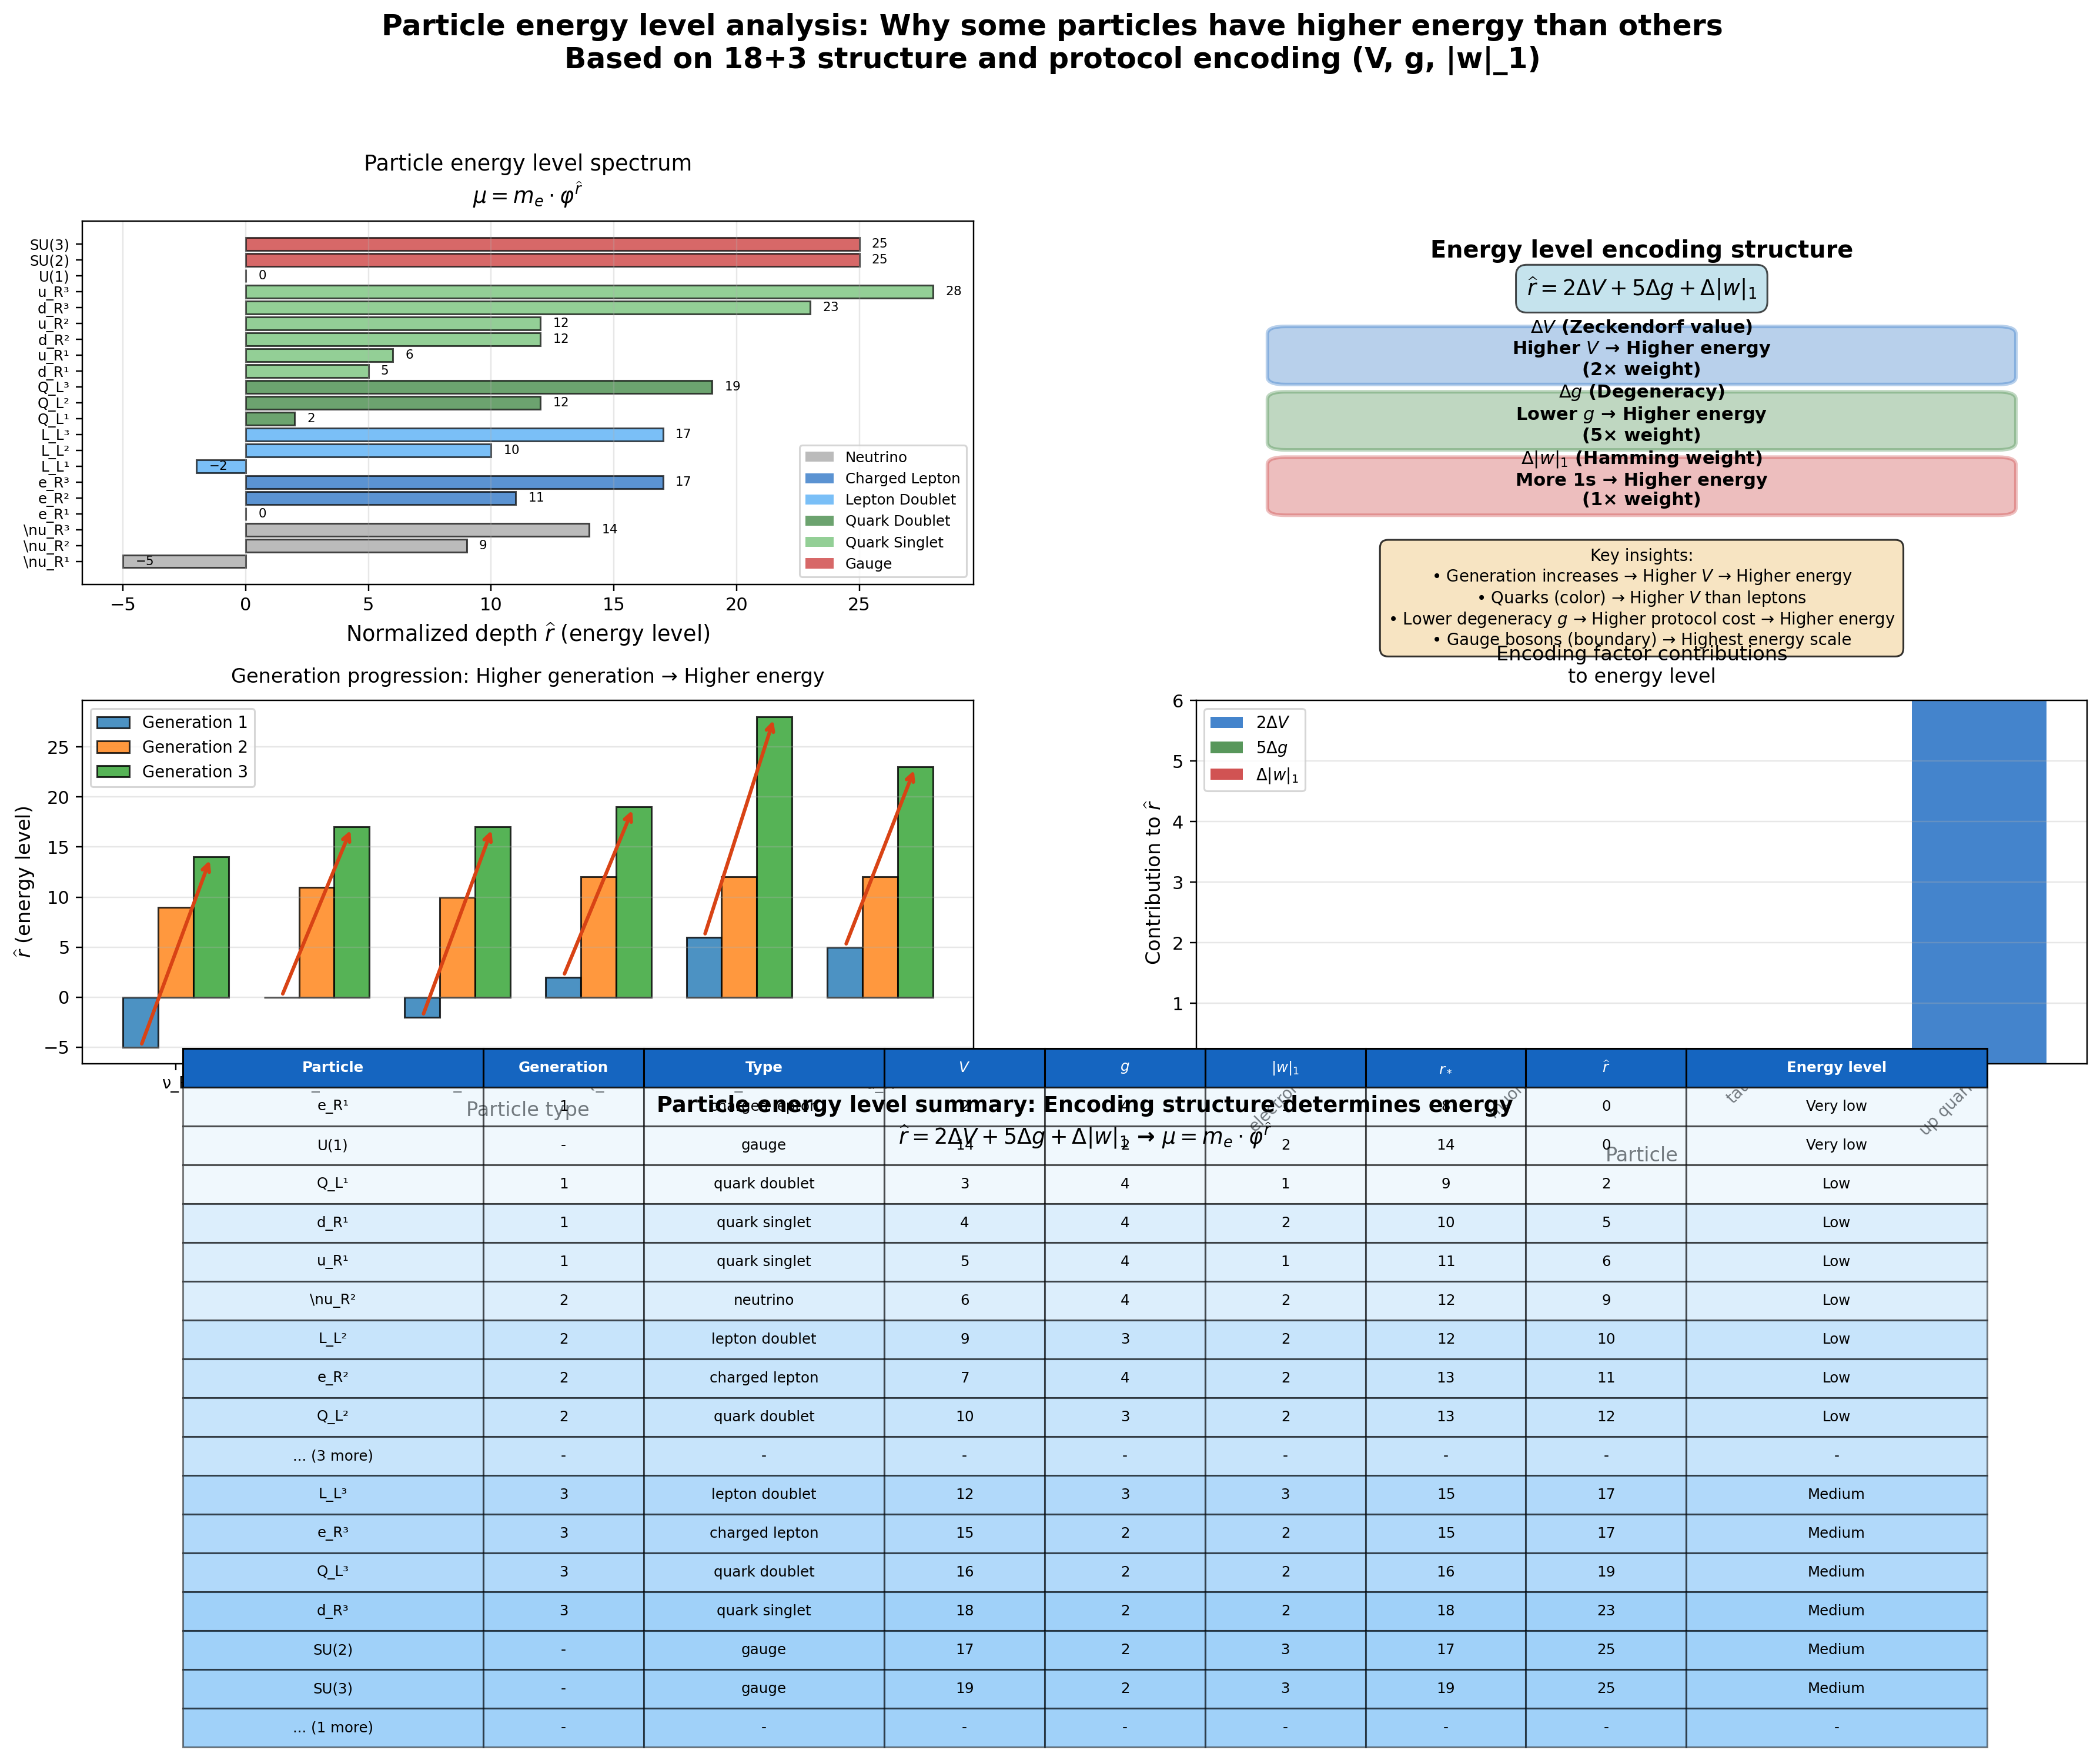
\includegraphics[width=0.98\textwidth]{figures/particle_energy_level_analysis.png}
\caption{Particle energy level analysis based on the 18+3 encoding structure: energy level spectrum (top-left), encoding factor contributions (top-right), generation progression (bottom-left), and comprehensive summary table (bottom). The normalized depth $\widehat{r}=2\Delta V+5\Delta g+\Delta|w|_1$ determines the energy scale via $\mu=m_e\cdot\varphi^{\widehat{r}}$. Key patterns: (1) Higher generation → Higher $V$ → Higher energy; (2) Quarks (color triplets) have higher $V$ than leptons at the same generation; (3) Lower degeneracy $g$ (fewer microstates sharing the label) corresponds to higher protocol cost and higher energy; (4) Gauge bosons (boundary types) appear at the highest energy scales. Generated by \texttt{scripts/fig\_particle\_energy\_level\_analysis.py}.}
\label{fig:particle_energy_level_analysis}
\end{figure}

\paragraph{Rigidity audits and matching-layer summaries (supplement).}
Bounded-coefficient rigidity searches, leave-one-out robustness diagnostics, and the quantized matching-layer tables are recorded in Appendix~\ref{app:mass_rigidity_details}.

\paragraph{Audit reading and failure criteria.}
\AuditTag The depth-coefficient closure is anchored on the scheme-stable charged-lepton set $\{\mu,\tau\}$ (Appendix~\ref{subsec:mass_depth_rigidity}); quark rows are treated as diagnostic matching inputs under a stated scheme convention rather than as scheme-independent rigidity anchors.
Operationally, the closure would be falsified \emph{within its stated hypothesis class} if (i) the bounded-integer minimizer for $(a,b,c)$ were not unique or did not stabilize across modest bound increases, or (ii) the matching-layer residuals required substantially finer denominators than the minimal dyadic quarter-step lattice to be compactly summarized (Appendix~\ref{subsec:mass_matching_layer}).
